% ============================================================
% UNIDAD 6: PREVENCIÓN DE ACCIDENTES Y SMS
% ============================================================
\clearpage
\section*{UNIDAD 6: PREVENCIÓN DE ACCIDENTES}
\subsection*{Riesgo, causalidad, investigación y gestión de la seguridad operacional (SMS)}

\begin{recuadro}
\textbf{Objetivo de la unidad:} comprender qué es el riesgo, cómo se producen los accidentes según
los distintos enfoques de causalidad, cómo se investigan, cómo funciona el ciclo de la seguridad
operacional y cómo se planifica y gestiona un \textbf{SMS} en un taller u organización
aeronáutica, incluyendo el análisis de los costos de los accidentes y de la prevención.
\end{recuadro}

% ------------------------------------------------------------
\section*{1. CONCEPTOS BÁSICOS}

\paragraph*{Seguridad operacional.} Según la OACI, es el estado en el que los riesgos asociados a
las actividades aeronáuticas se reducen y controlan a un \textbf{nivel aceptable}. No significa
``cero riesgo'' (eso no existe), sino riesgo \textbf{gestionado}.

\begin{center}
\small
\begin{tabular}{|p{0.18\linewidth}|p{0.42\linewidth}|p{0.28\linewidth}|}
\hline
\textbf{Concepto} & \textbf{Definición} & \textbf{Ejemplo} \\ \hline
\textbf{Peligro} & Condición u objeto que podría causar un accidente o daño. & Un piso con
fluido hidráulico derramado. \\ \hline
\textbf{Consecuencia} & El resultado posible del peligro. & Una caída. \\ \hline
\textbf{Riesgo} & Combinación de la \textbf{probabilidad} de la consecuencia y su
\textbf{gravedad}. & Probable y con lesiones leves. \\ \hline
\end{tabular}
\end{center}

\paragraph*{Accidente, incidente grave e incidente (Anexo 13).}
\begin{itemize}
  \item \textbf{Accidente:} suceso relacionado con la operación de una aeronave en el que una
        persona muere o sufre \textbf{lesiones graves}, o la aeronave sufre \textbf{daños o roturas
        estructurales} que afectan su resistencia, su funcionamiento o sus características de
        vuelo, o la aeronave desaparece o es inaccesible.
  \item \textbf{Incidente grave:} incidente en el que las circunstancias indican que hubo una
        \textbf{alta probabilidad de accidente} (por ejemplo, una casi colisión, una salida de pista
        sin daños, un incendio a bordo controlado).
  \item \textbf{Incidente:} todo suceso, distinto del accidente, que afecta o puede afectar la
        seguridad de las operaciones.
\end{itemize}

% ------------------------------------------------------------
\section*{2. LAS CAUSAS DE LOS ACCIDENTES: ENFOQUES DE CAUSALIDAD}

\subsubsection*{2.1. Enfoque tradicional}
Busca \textbf{la causa} (generalmente, la última persona que actuó: ``error del piloto'', ``error
del mecánico'') y al \textbf{culpable}. El modelo del \textbf{dominó} (Heinrich, años treinta)
representa el accidente como una cadena de fichas que caen una tras otra: si se quita una, el
accidente no ocurre.

\paragraph*{La pirámide de accidentes.} Los estudios de Heinrich y luego de Frank Bird mostraron
que por cada accidente grave hay muchos incidentes menores y cientos de ``casi accidentes'' y
condiciones inseguras. Conclusión: si se reportan y corrigen los sucesos de la base, se previenen
los de la punta.

\begin{center}
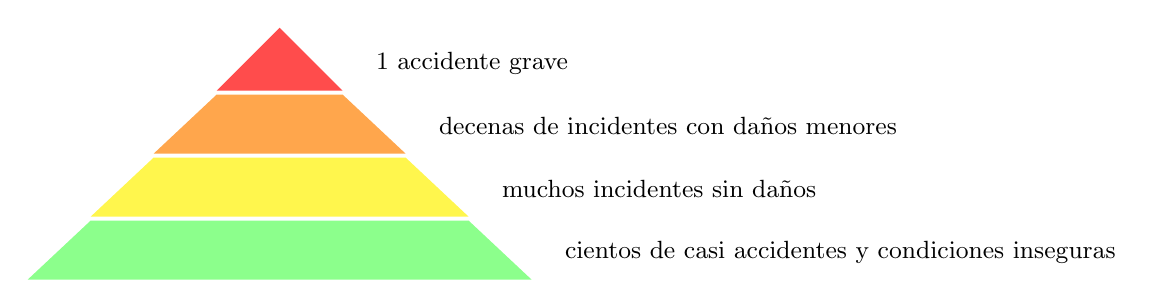
\begin{tikzpicture}[every node/.style={font=\small}]
  \fill[red!70] (0,3.2) -- (-0.8,2.4) -- (0.8,2.4) -- cycle;
  \fill[orange!70] (-0.8,2.35) -- (0.8,2.35) -- (1.6,1.6) -- (-1.6,1.6) -- cycle;
  \fill[yellow!70] (-1.6,1.55) -- (1.6,1.55) -- (2.4,0.8) -- (-2.4,0.8) -- cycle;
  \fill[green!45] (-2.4,0.75) -- (2.4,0.75) -- (3.2,0) -- (-3.2,0) -- cycle;
  \node[anchor=west] at (1.1,2.75) {1 accidente grave};
  \node[anchor=west] at (1.9,1.95) {decenas de incidentes con daños menores};
  \node[anchor=west] at (2.7,1.15) {muchos incidentes sin daños};
  \node[anchor=west] at (3.5,0.35) {cientos de casi accidentes y condiciones inseguras};
\end{tikzpicture}
\end{center}

\subsubsection*{2.2. Enfoque organizacional: el modelo de Reason (``queso suizo'')}
James Reason propuso que los accidentes ocurren cuando se \textbf{alinean los agujeros} de varias
\textbf{defensas} (capas de queso): la organización, la supervisión, las condiciones de trabajo y
las acciones de las personas.
\begin{itemize}
  \item \textbf{Fallas activas:} errores o violaciones de quienes están en contacto directo con la
        aeronave; su efecto es inmediato.
  \item \textbf{Condiciones latentes:} decisiones tomadas lejos del lugar y del momento del
        accidente (presupuestos, turnos, diseño de procedimientos, falta de instrucción) que
        ``esperan'' a que alguien se equivoque.
\end{itemize}

\begin{center}
\begin{tikzpicture}[every node/.style={font=\footnotesize, align=center}]
  \foreach \x/\t in {0/Decisiones de\\ la organización, 2.6/Supervisión\\ deficiente,
                     5.2/Condiciones\\ de trabajo, 7.8/Acto inseguro\\ (falla activa)} {
    \fill[yellow!55, draw=orange!80!black, thick, rounded corners=3pt]
      (\x,0) -- (\x+0.6,0.45) -- (\x+0.6,3.3) -- (\x,2.85) -- cycle;
    \node at (\x+0.3,-0.55) {\t};
  }
  \foreach \x in {0,2.6,5.2,7.8} {
    \fill[white, draw=orange!80!black] (\x+0.3,1.75) ellipse (0.12 and 0.22);
    \fill[white, draw=orange!80!black] (\x+0.3,2.6) ellipse (0.09 and 0.15);
  }
  \fill[white, draw=orange!80!black] (0.3,0.9) ellipse (0.1 and 0.18);
  \fill[white, draw=orange!80!black] (5.5,1.0) ellipse (0.1 and 0.18);
  \draw[-{Stealth}, very thick, red] (-1.2,1.75) -- (10.0,1.75);
  \node[red, anchor=west] at (10.05,1.75) {\textbf{ACCIDENTE}};
  \node[red, anchor=east] at (-1.25,1.75) {Peligro};
\end{tikzpicture}
\end{center}

\subsubsection*{2.3. Enfoque sistémico o moderno}
Ve a la aviación como un \textbf{sistema complejo}: personas, tecnología, organizaciones y
regulaciones en interacción. Los accidentes surgen de la combinación de factores normales que, en
conjunto, se vuelven peligrosos, y de la ``deriva'' de las prácticas reales respecto de lo
escrito. Pone el foco en entender cómo el trabajo \textbf{se hace realmente}, en aprender también
de lo que sale bien y en fortalecer la \textbf{resiliencia} de la organización.

\begin{center}
\small
\begin{tabular}{|p{0.22\linewidth}|p{0.33\linewidth}|p{0.33\linewidth}|}
\hline
 & \textbf{Enfoque tradicional} & \textbf{Enfoque moderno} \\ \hline
Pregunta & ¿Quién tuvo la culpa? & ¿Por qué tuvo sentido lo que hicieron? ¿Qué falló en el
sistema? \\ \hline
Causa & Una, la última & Muchas, organizacionales y latentes \\ \hline
Respuesta & Sancionar, reentrenar a la persona & Corregir condiciones, procedimientos y
organización \\ \hline
Información & Se oculta por miedo & Se reporta (cultura justa) \\ \hline
Actuación & Reactiva (después del accidente) & Proactiva y predictiva (antes) \\ \hline
\end{tabular}
\end{center}

% ------------------------------------------------------------
\section*{3. LA INVESTIGACIÓN DE ACCIDENTES}

El \textbf{Anexo 13} de la OACI establece que el \textbf{único objetivo} de la investigación de
accidentes e incidentes es \textbf{prevenir} futuros accidentes, y \textbf{no determinar culpas ni
responsabilidades}. En la Argentina la realiza la \textbf{Junta de Seguridad en el Transporte
(JST)}, independiente de la autoridad que regula (la ANAC) y de la Justicia.

\paragraph*{Etapas.} Notificación del suceso; preservación de las evidencias; trabajo de campo
(restos, registradores de vuelo, documentación, testigos); análisis; informe preliminar;
\textbf{informe final} con conclusiones y \textbf{recomendaciones de seguridad} dirigidas a
quienes pueden corregir el problema (autoridad, fabricante, operador, taller).

\paragraph*{El aporte del mantenimiento.} En toda investigación se revisan los registros de
mantenimiento, el cumplimiento de directivas y la historia de los componentes. Un registro
completo y veraz protege a la aviación y al propio técnico.

% ------------------------------------------------------------
\section*{4. EL CICLO DE LA SEGURIDAD OPERACIONAL Y LA GESTIÓN DE RIESGOS}

\begin{center}
\begin{tikzpicture}[every node/.style={font=\small, align=center},
  e/.style={draw=ppAzul, very thick, rounded corners, fill=ppAzul!8, text width=2.9cm,
  minimum height=1.05cm}]
  \node[e] (a) at (90:2.3) {\textbf{1. Identificar}\\ peligros};
  \node[e] (b) at (18:2.9) {\textbf{2. Evaluar}\\ el riesgo};
  \node[e] (c) at (-54:2.6) {\textbf{3. Mitigar}\\ (defensas)};
  \node[e] (d) at (-126:2.6) {\textbf{4. Monitorear}\\ indicadores};
  \node[e] (f) at (162:2.9) {\textbf{5. Revisar}\\ y mejorar};
  \draw[-{Stealth}, thick] (a) to[bend left=15] (b);
  \draw[-{Stealth}, thick] (b) to[bend left=15] (c);
  \draw[-{Stealth}, thick] (c) to[bend left=15] (d);
  \draw[-{Stealth}, thick] (d) to[bend left=15] (f);
  \draw[-{Stealth}, thick] (f) to[bend left=15] (a);
\end{tikzpicture}
\end{center}

\subsubsection*{4.1. Identificación de peligros}
Fuentes \textbf{reactivas} (análisis de accidentes e incidentes ocurridos), \textbf{proactivas}
(reportes voluntarios, auditorías, inspecciones, encuestas) y \textbf{predictivas} (análisis de
datos para detectar tendencias antes de que ocurra algo).

\subsubsection*{4.2. Evaluación del riesgo: la matriz}
\begin{center}
\small
\begin{tabular}{|p{0.30\linewidth}|c|c|c|c|c|}
\hline
\textbf{Probabilidad} $\backslash$ \textbf{Gravedad} & \textbf{A} Catastrófico & \textbf{B}
Peligroso & \textbf{C} Grave & \textbf{D} Leve & \textbf{E} Insignificante \\ \hline
\textbf{5} Frecuente & \textbf{5A} & \textbf{5B} & \textbf{5C} & 5D & 5E \\ \hline
\textbf{4} Ocasional & \textbf{4A} & \textbf{4B} & 4C & 4D & 4E \\ \hline
\textbf{3} Remoto & \textbf{3A} & 3B & 3C & 3D & \textit{3E} \\ \hline
\textbf{2} Improbable & 2A & 2B & 2C & \textit{2D} & \textit{2E} \\ \hline
\textbf{1} Sumamente improbable & 1A & \textit{1B} & \textit{1C} & \textit{1D} & \textit{1E} \\
\hline
\end{tabular}
\end{center}
\begin{itemize}
  \item \textbf{Intolerable} (en negrita: 5A, 5B, 5C, 4A, 4B, 3A): no se puede operar así; hay que
        detener o mitigar de inmediato.
  \item \textbf{Tolerable} (normal): se acepta solo con medidas de mitigación y aprobación de la
        dirección.
  \item \textbf{Aceptable} (en cursiva): se puede operar; se sigue monitoreando.
\end{itemize}

\subsubsection*{4.3. Mitigación: la jerarquía de controles}
De más a menos eficaz: \textbf{eliminar} el peligro; \textbf{sustituir} por algo menos
peligroso; \textbf{controles de ingeniería} (barandas, protecciones, alarmas); \textbf{controles
administrativos} (procedimientos, capacitación, señalización); \textbf{elementos de protección
personal}.

% ------------------------------------------------------------
\section*{5. EL SISTEMA DE GESTIÓN DE LA SEGURIDAD OPERACIONAL (SMS)}

El \textbf{SMS} (\textit{Safety Management System}) es un enfoque sistemático para gestionar la
seguridad operacional, que incluye la estructura organizacional, las responsabilidades, las
políticas y los procedimientos necesarios. Lo exige el \textbf{Anexo 19} de la OACI a los
operadores, talleres de mantenimiento, organizaciones de diseño y fabricación, centros de
instrucción, proveedores de servicios de tránsito aéreo y aeródromos, \textbf{ajustado a su tamaño
y complejidad}. La guía principal es el \textbf{Doc 9859} de la OACI.

\subsubsection*{5.1. El marco del SMS: 4 componentes y 12 elementos}
\begin{center}
\small
\begin{tabular}{|p{0.30\linewidth}|p{0.60\linewidth}|}
\hline
\textbf{Componente} & \textbf{Elementos} \\ \hline
\textbf{1. Política y objetivos de seguridad operacional} & 1.1 Compromiso de la dirección. \newline
1.2 Obligación de rendición de cuentas y responsabilidades. \newline
1.3 Designación del personal clave de seguridad operacional. \newline
1.4 Coordinación de la planificación de respuesta ante emergencias. \newline
1.5 Documentación del SMS. \\ \hline
\textbf{2. Gestión de riesgos de seguridad operacional} & 2.1 Identificación de peligros. \newline
2.2 Evaluación y mitigación de riesgos. \\ \hline
\textbf{3. Aseguramiento de la seguridad operacional} & 3.1 Observación y medición del
rendimiento en materia de seguridad operacional. \newline
3.2 Gestión del cambio. \newline
3.3 Mejora continua del SMS. \\ \hline
\textbf{4. Promoción de la seguridad operacional} & 4.1 Instrucción y educación. \newline
4.2 Comunicación de la seguridad operacional. \\ \hline
\end{tabular}
\end{center}

\subsubsection*{5.2. Indicadores y metas}
Un SMS se mide con \textbf{indicadores de rendimiento} (SPI), por ejemplo: cantidad de reportes
voluntarios por mes, errores de mantenimiento detectados en inspección, fallas repetitivas,
hallazgos de auditoría abiertos. A cada indicador se le fijan \textbf{metas} (SPT) y niveles de
alerta.

\subsubsection*{5.3. El Programa Estatal de Seguridad Operacional (SSP)}
Así como cada organización tiene su SMS, cada \textbf{Estado} debe tener un \textbf{SSP}: el
conjunto de normas y actividades con las que gestiona la seguridad de toda su aviación civil
(regulación, vigilancia, investigación, promoción) y acepta y supervisa los SMS de las
organizaciones.

\subsubsection*{5.4. La cultura de seguridad}
Ningún sistema funciona sin una \textbf{cultura de seguridad}: una organización donde la gente
\textbf{informa} lo que ve (cultura de reporte), se la trata con \textbf{justicia}, la
organización \textbf{aprende} de sus errores y la dirección da el ejemplo. La seguridad no es un
departamento: es la forma de trabajar de todos.

% ------------------------------------------------------------
\section*{6. LOS COSTOS DE LOS ACCIDENTES Y DE LA SEGURIDAD}

\begin{itemize}
  \item \textbf{Costos directos:} daños a la aeronave, lesiones, indemnizaciones; en general los
        cubre el seguro.
  \item \textbf{Costos indirectos:} los que no cubre el seguro, y suelen ser \textbf{mucho
        mayores} (la ``parte oculta del iceberg''): pérdida de ingresos mientras la aeronave no
        vuela, reemplazo de equipos, horas de investigación y trámites, multas, aumento de las
        primas de seguro, pérdida de clientes y de reputación, efecto en el personal.
  \item \textbf{Costos de los incidentes:} aunque no haya víctimas, un incidente genera
        reparaciones, demoras, cancelaciones y AOG.
  \item \textbf{Costos de la seguridad:} instrucción, personal de calidad y SMS, herramientas,
        repuestos, tiempo de inspección. Son una \textbf{inversión}: previenen pérdidas muy
        superiores.
\end{itemize}
\textit{``Si usted piensa que la seguridad es cara, pruebe con un accidente.''}

% ------------------------------------------------------------
\section*{7. CASOS PARA ANALIZAR}

\begin{center}
\footnotesize
\begin{tabular}{|p{0.22\linewidth}|p{0.40\linewidth}|p{0.28\linewidth}|}
\hline
\textbf{Caso} & \textbf{Qué pasó} & \textbf{Tema clave} \\ \hline
Tenerife (España), 27/3/1977 & Dos Boeing 747 chocaron en la pista con niebla; 583 muertos, el
peor accidente de la historia de la aviación. & Comunicación, jerarquía en cabina, origen del
CRM. \\ \hline
American 191 (Chicago), 25/5/1979 & Un DC-10 perdió un motor al despegar; el pilón había sido
dañado en mantenimiento por un procedimiento no aprobado para ahorrar tiempo. & Procedimientos
``alternativos'', presión de tiempo. \\ \hline
Aloha 243 (Hawái), 28/4/1988 & Un Boeing 737 con muchísimos ciclos perdió parte del techo del
fuselaje en vuelo; murió una tripulante. & Fatiga y corrosión, eficacia de las inspecciones. \\
\hline
Continental Express 2574 (Texas), 11/9/1991 & Trabajo incompleto en el estabilizador no
comunicado en el pase de turno. & Pase de turno, MRM. \\ \hline
British Airways 5390 (R. Unido), 10/6/1990 & Parabrisas instalado con tornillos equivocados. &
Número de parte, verificación. \\ \hline
Austral 2553 (Fray Bentos, Uruguay), 10/10/1997 & Un DC-9 se estrelló tras una indicación
errónea de velocidad por hielo en el sistema pitot y la extensión de los slats a alta velocidad;
74 muertos. & Instrumentos, entrenamiento, factores humanos. \\ \hline
LAPA 3142 (Aeroparque), 31/8/1999 & Un Boeing 737 intentó despegar sin los flaps extendidos; la
alarma sonó y no fue atendida; 65 muertos. & Factores organizacionales, cultura de la empresa
y vigilancia del Estado. \\ \hline
Alaska 261 (California), 31/1/2000 & Un MD-83 perdió el control por el desgaste del tornillo
del estabilizador horizontal, con lubricación insuficiente e intervalos de inspección
extendidos; 88 muertos. & Programa de mantenimiento, intervalos. \\ \hline
Southwest 1380 (EE.\,UU.), 17/4/2018 & Un álabe del fan se rompió por fatiga; los restos dañaron
el fuselaje; murió una pasajera. & Inspecciones de motores, AD. \\ \hline
Alaska 1282 (Portland), 5/1/2024 & En un 737 MAX 9 se desprendió en vuelo un tapón de puerta al
que le faltaban los pernos tras un trabajo en fábrica; sin víctimas fatales. & Control de
calidad, documentación de remociones. \\ \hline
Washington DC, 29/1/2025 & Colisión en vuelo entre un avión regional y un helicóptero militar
cerca del aeropuerto Reagan; 67 muertos. & Gestión del tránsito aéreo, separación, riesgos
conocidos no gestionados. \\ \hline
UPS 2976 (Louisville), 4/11/2025 & Un MD-11F perdió el motor izquierdo con su pilón al despegar;
14 muertos (ver Unidad 2). & Aeronavegabilidad continuada, información del fabricante. \\
\hline
\end{tabular}
\end{center}

\paragraph*{Material audiovisual sugerido.}
\begin{itemize}
  \item La serie documental \textbf{\textit{Mayday: Catástrofes aéreas}} (\textit{Air Crash
        Investigation}), que reconstruye muchos de estos casos con la información de los
        informes oficiales (Tenerife, Aloha 243, Alaska 261, British Airways 5390, entre otros).
  \item La película argentina \textbf{\textit{Whisky Romeo Zulu}} (2004), de Enrique Piñeyro,
        ex piloto de LAPA, sobre el contexto organizacional del accidente de LAPA 3142.
  \item Los \textbf{informes finales} de la JST y de la NTSB, disponibles en sus sitios web.
\end{itemize}

% ------------------------------------------------------------
\section*{8. ACTIVIDADES DE LA UNIDAD}
\begin{enumerate}
  \item \textbf{Tradicional vs.\ moderno:} elegir un caso de la tabla y escribir dos conclusiones:
        una como la escribiría el enfoque tradicional (``la causa fue...'') y otra con el enfoque
        moderno (factores latentes y organizacionales). ¿Cuál previene mejor?
  \item \textbf{Queso suizo:} analizar un caso con el modelo de Reason, identificando las fallas
        activas y las condiciones latentes en cada capa.
  \item \textbf{Informe de la JST:} leer un informe final de la JST de un accidente de aviación
        general y resumir sus recomendaciones de seguridad.
  \item \textbf{Matriz de riesgos del taller:} identificar diez peligros del taller de la escuela,
        evaluarlos en la matriz y proponer medidas según la jerarquía de controles.
  \item \textbf{Simulación del ciclo:} implementar una medida preventiva en el taller (por ejemplo,
        un tablero de sombra para herramientas) y medir durante un mes un indicador.
  \item \textbf{Informe de costos:} con un caso hipotético de un incidente de mantenimiento (por
        ejemplo, una herramienta olvidada que dañó un motor), estimar los costos directos e
        indirectos y redactar un informe que justifique la inversión en prevención.
\end{enumerate}
